Le projet sera géré selon la méthodologie \textbf{Scrum}  \ref{sec:presentation_scrum}, favorisant une approche agile avec des cycles itératifs appelés \textbf{sprints}. Le \textbf{Product Owner}, l’\textbf{équipe de développement} et le \textbf{Scrum Master} collaboreront pour assurer une livraison progressive des fonctionnalités clés.

\subsection*{Acteurs Scrum et Missions}
\begin{longtable}{|m{3cm}|m{8cm}|m{2cm}|}
\hline
\textbf{Rôle} & \textbf{Mission} & \textbf{Acteur} \\
\hline
\endfirsthead
\hline
\textbf{Rôle} & \textbf{Mission} & \textbf{Acteur} \\
\hline
\endhead
% \hline
\endfoot
Product Owner & 
- Définir et prioriser les fonctionnalités du produit (Product Backlog). \newline
- Assurer que l'équipe travaille sur les fonctionnalités les plus importantes. \newline
- Valider les livrables à la fin de chaque sprint. &
Pr Ammeri Charfeddine \\
\hline
Équipe de Développement & 
- Concevoir, développer et tester les fonctionnalités du produit. \newline
- Participer aux réunions de planification et de revue de sprint. \newline
- Assurer la qualité du code et des livrables. &
Zaibi Racha \\
\hline
Scrum Master & 
- Faciliter les réunions Scrum (Daily Stand-up, Sprint Planning, Sprint Review, Retrospective). \newline
- Supprimer les obstacles qui empêchent l'équipe de progresser. \newline
- Assurer que l'équipe suit les principes Scrum. &
Ouni Ghada\\
\hline
\caption{Acteurs du projet} 
\end{longtable}

\subsection*{Organisation du Backlog}
Le \textbf{Product Backlog} géré via ClickUp \ref{subsec:outils_scrum} regroupe l’ensemble des fonctionnalités à développer pour le système. Chacune est formulée sous forme de \textit{User Story}, garantissant une approche centrée sur l’utilisateur.

Chaque fonctionnalité sera développée et livrée en plusieurs \textbf{sprints}, selon les priorités établies par le \textit{Product Owner}. Elles sont classées selon la méthode \textbf{MoSCoW}, qui définit les niveaux de priorité pour chaque tâche.

\section*{Backlog du Projet}
\label{sec:backlog_projet} 
% Le \textbf{Backlog} est un élément central de la méthodologie \textbf{Scrum}. Il regroupe toutes les spécifications fonctionnelles et techniques du produit.

\begin{longtable}{|c|p{9cm}|c|}
    \hline
    \textbf{ID} & \textbf{Tâche} & \textbf{Priority} \\
    \hline
    \endfirsthead
    \hline
    \textbf{ID} & \textbf{Tâche} & \textbf{Priority} \\
    \hline
    \endhead
    % \hline
    \endfoot
    M-01& Détection et reconnaissance des valeurs vitales via OCR pour les moniteurs des signes vitaux. & M \\
    \hline
    M-02 & Génération et gestion des alertes en fonction des seuils prédéfinis. & M \\
    \hline
    M-03 & Envoi d’alertes aux médecins et infirmiers via notifications push (FCM) et e-mail. & M \\
    \hline
    M-04 & Interface web et mobile pour visualiser les données des patients et gérer les alertes. & M \\
    \hline
    M-05 & Authentification et gestion des utilisateurs (médecins, infirmiers, administrateurs). & M \\
    \hline
    M-06 & Stockage et historique des données. & M \\
    \hline
    M-07 & Conformité aux réglementations médicales (sécurité des données). & M \\
    \hline
    S-02 & Configuration des seuils d’alerte personnalisés par patient. & S \\
    \hline
    S-03 & Gestion des horaires de filtrage des alertes pour le personnel médical. & S \\
    \hline
    S-04 & Interface d’administration pour configurer les seuils d’alerte et gérer les utilisateurs. & S \\
    \hline
    S-05 & Notifications push. & S \\
    \hline
    C-04 & Support multilingue pour l’interface utilisateur. & C \\
    \hline
    C-05 & Gestion des alertes par priorité (critique, moyen, faible). & C \\
    \hline
    C-06 & Historique des alertes avec possibilité de filtrage par date, patient, ou type d’alerte. & C \\
    \hline
    % W-01 & Intégration avec des systèmes de gestion hospitalière (HIS) tiers. &W \\
    % % \hline
    % W-02 & Déploiement du système dans plusieurs hôpitaux ou centres médicaux. &W \\
    % \hline
    W-03 & Analyse avancée des données avec intelligence artificielle pour le diagnostic médical. &W \\
    % \hline
    % W-04 & Support pour d’autres langues de programmation ou frameworks non prévus initialement. &W \\
    % \hline
    % W-05 & Développement d’une application desktop en plus des interfaces web et mobile. &W \\
    \hline
\caption{Backlog du Projet avec Priorités MoSCoW} 
\label{tab:backlog_moscow}
\end{longtable}
\section*{Clé des Priorités MoSCoW}
\begin{itemize}
    \item \textbf{M (Must)} : Tâches critiques nécessaires au bon fonctionnement du système.
    \item \textbf{S (Should)} : Tâches importantes qui apportent une valeur significative mais ne sont pas essentielles pour la première version.
    \item \textbf{C (Could)} : Fonctionnalités optionnelles pouvant être ajoutées si le temps et les ressources le permettent.
    \item \textbf{W (Won't Have)} : Tâches hors du périmètre de la phase actuelle du projet.
\end{itemize}

% \subsection{Diagramme des cas d’utilisation global}
% Montrez les prototypes initiaux pour les interfaces du système (par exemple, visualisation des données, gestion des alertes).

\begin{figure}[H]
    \centering
    \begin{minipage}{1\textwidth}
        \centering
        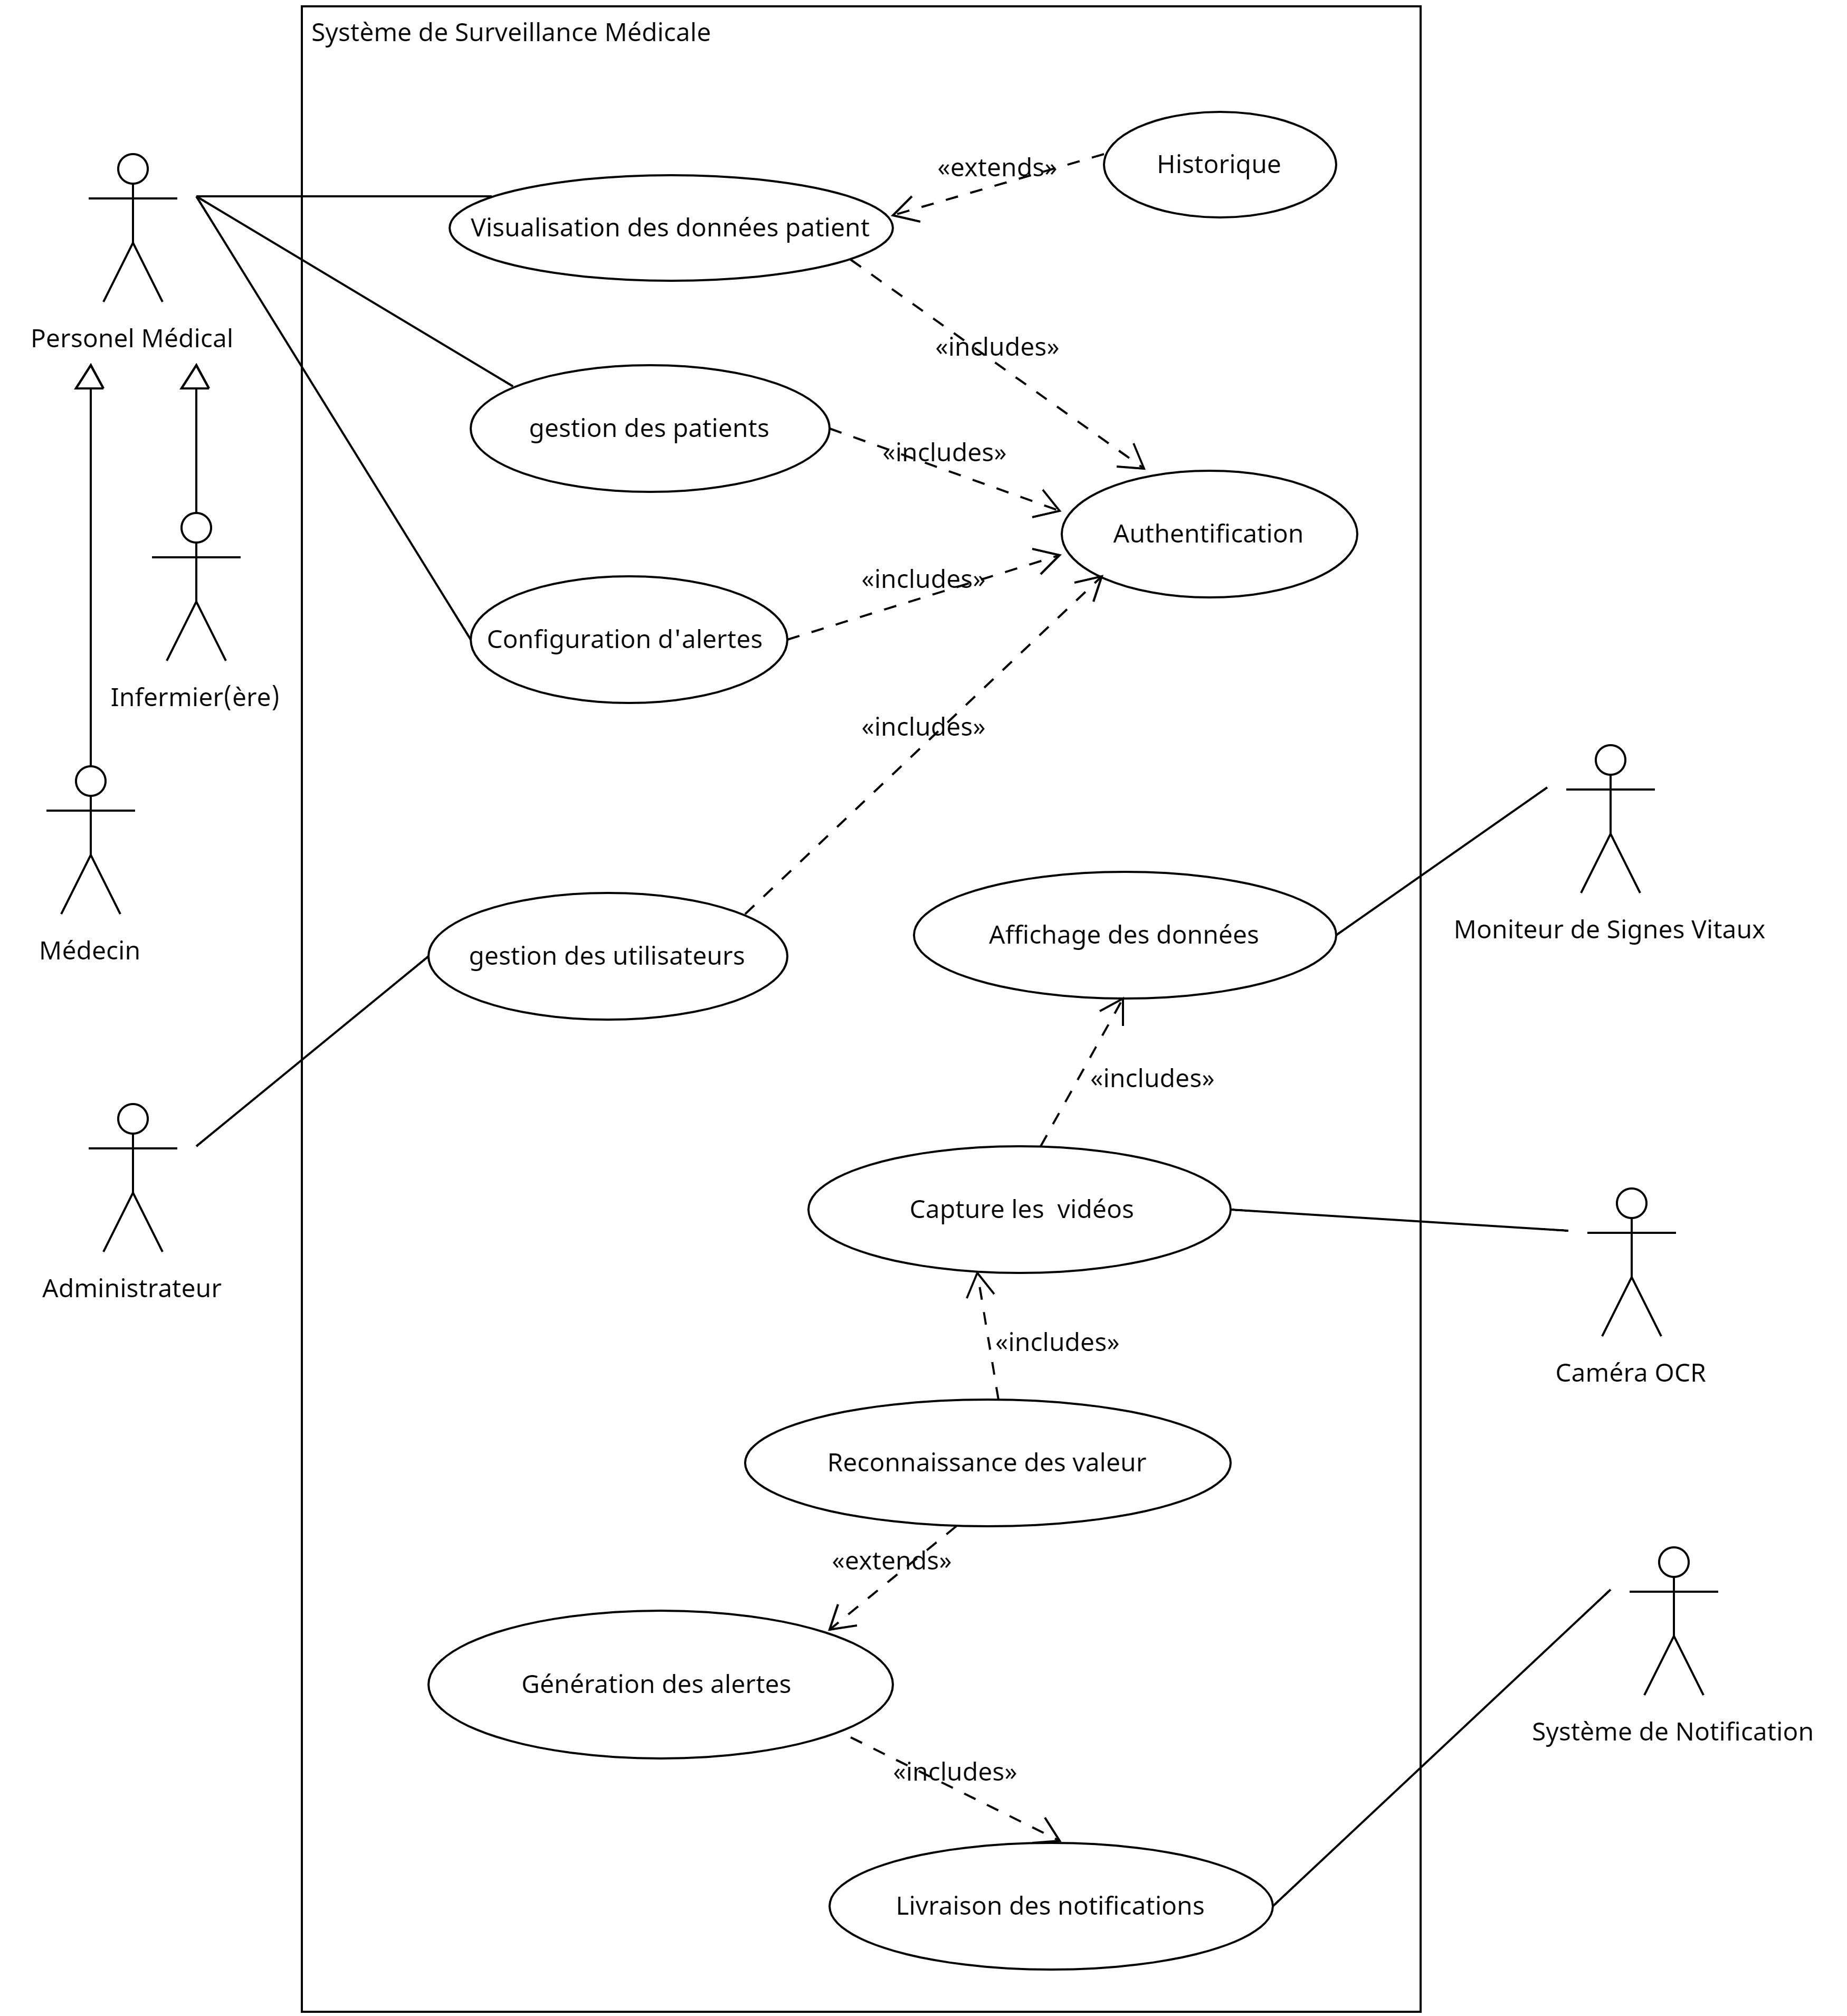
\includegraphics[width=\linewidth]{chapter4/sections/diagrams/use_case.png}
        \caption{Diagramme des cas d’utilisation global}
    \end{minipage}
\end{figure} 
\subsection{Planification des sprints}

Une fois le backlog du produit finalisé, nous avons organisé la réunion de planification de sprint. L'objectif de cette réunion était de construire le backlog de sprint en se basant sur le backlog de produit défini par le Product Owner. À l'issue de cette réunion, nous avons identifié les durées prévisionnelles du travail à effectuer pour chaque sprint. Pour ce projet, nous avons divisé le travail en trois sprints, chacun d'une durée de 3 semaines, regroupés en une seule release. La figure 2.3 illustre la répartition des sprints pour notre système.

\medskip

\textbf{Plan des sprints :}

\begin{itemize}
    \item \textbf{Sprint 1 : Collecte de données basée sur caméra}
    \begin{itemize}
        \item \textbf{Objectif} : Mettre en place un système de collecte de données à partir des moniteurs des signes vitaux en utilisant des caméras et des techniques de reconnaissance optique de caractères (OCR).
        \item \textbf{Deliverables} :
            \begin{itemize}
                \item Intégration de la caméra IP avec le système.
                \item Pipeline OCR pour extraire les valeurs vitales (fréquence cardiaque, pression artérielle, SpO2).
            \end{itemize}
        \item \textbf{Durée} : 3 semaines.
        \item \textbf{Tâches clés} :
            \begin{itemize}
                \item Configuration des caméras IP (montage fixe, résolution 1080p).
                \item Installation et configuration des logiciels OCR (OpenCV, Tesseract).
                \item Développement du pipeline de prétraitement et extraction d'images.
            \end{itemize}
        \item \textbf{Critères d'acceptation} :
            \begin{itemize}
                \item Le pipeline OCR extrait les valeurs vitales avec une précision d'au moins 95\%, validée par comparaison avec 10 lectures manuelles.
                \item Les images sont traitées avec une latence inférieure à 1 seconde par frame dans 100\% des tests.
                \item Le pipeline est compatible avec les moniteurs Mindray et Edan, testé sur au moins 5 scénarios différents.
            \end{itemize}
        \item \textbf{Risques} :
            \begin{itemize}
                \item Mauvaise qualité d'image affectant la précision de l'OCR.
                \item Solution : Utilisation de caméras haute résolution et optimisation du prétraitement des images avec OpenCV.
            \end{itemize}
    \end{itemize}

    \item \textbf{Sprint 2 : Validation des données et gestion des alertes}
    \begin{itemize}
        \item \textbf{Objectif} : Valider les données collectées et développer un système de gestion des alertes basé sur des seuils prédéfinis.
        \item \textbf{Deliverables} :
            \begin{itemize}
                \item Validation des données OCR par rapport aux données réelles.
                \item Module de gestion des alertes avec seuils prédéfinis.
                \item Notifications push via Firebase Cloud Messaging (FCM).
            \end{itemize}
        \item \textbf{Durée} : 3 semaines.
        \item \textbf{Tâches clés} :
            \begin{itemize}
                \item Tests de validation des données extraites (comparaison avec lectures manuelles).
                \item Développement du module de détection des anomalies basé sur des seuils.
                \item Intégration de FCM pour les notifications push sur mobile.
            \end{itemize}
        \item \textbf{Critères d'acceptation} :
            \begin{itemize}
                \item Les données extraites correspondent aux valeurs réelles avec une précision de 98\% dans 20 tests.
                \item Les alertes sont déclenchées en moins de 2 secondes lorsque les seuils sont dépassés (e.g., fréquence cardiaque > 120 bpm).
                \item Les notifications push sont reçues avec un taux de succès de 99\% sur Android et iOS dans un environnement de test.
            \end{itemize}
        \item \textbf{Dépendances} : Données collectées et pipeline OCR fonctionnel du Sprint 1.
        \item \textbf{Risques} :
            \begin{itemize}
                \item Retards dans la validation des données en raison d'erreurs OCR.
                \item Solution : Ajout de tests unitaires et manuels supplémentaires pour l'OCR.
            \end{itemize}
    \end{itemize}

    \item \textbf{Sprint 3 : Interface utilisateur et stockage des données}
    \begin{itemize}
        \item \textbf{Objectif} : Développer une interface utilisateur pour visualiser les données et alertes, et mettre en place le stockage des données.
        \item \textbf{Deliverables} :
            \begin{itemize}
                \item Tableau de bord web (React) pour afficher les données vitales et alertes.
                \item Application mobile (Flutter) pour les notifications et la consultation.
                \item Base de données MySQL pour stocker les données et historiques.
            \end{itemize}
        \item \textbf{Durée} : 3 semaines.
        \item \textbf{Tâches clés} :
            \begin{itemize}
                \item Conception et développement du tableau de bord web avec React.
                \item Développement de l'application mobile Flutter avec intégration FCM.
                \item Configuration de la base de données MySQL pour le stockage des données et alertes.
            \end{itemize}
        \item \textbf{Critères d'acceptation} :
            \begin{itemize}
                \item Le tableau de bord affiche les données vitales et alertes en temps réel avec un rafraîchissement toutes les 5 secondes, validé par 5 utilisateurs médicaux.
                \item L'application mobile permet la consultation des alertes avec une ergonomie validée par 3 infirmiers (aucun problème d'utilisabilité signalé).
                \item Les données sont stockées dans MySQL avec 100\% d'intégrité (aucune perte de données dans 50 tests).
            \end{itemize}
        \item \textbf{Dépendances} : Données validées et système d'alertes du Sprint 2.
        \item \textbf{Risques} :
            \begin{itemize}
                \item Complexité dans l'intégration des interfaces web et mobile.
                \item Solution : Prototypage préliminaire et tests d'utilisabilité itératifs.
            \end{itemize}
    \end{itemize}
\end{itemize} 
% \subsection{Prototypage des interfaces}
% Montrez les prototypes initiaux pour les interfaces du système (par exemple, visualisation des données, gestion des alertes).
 

